\documentclass{article}
\usepackage[utf8]{inputenc}
\usepackage[english,russian]{babel}
\usepackage{hyperref}
\usepackage{graphicx}
\usepackage[scale=0.75]{geometry}

\title{Лабораторная работа #1}
\author{Крухмалев Константин,Рашо Елизавета,Фролова Дарья, М34371}

\begin{document}


\maketitle


\href{https://github.com/Konstantin343/optimization-methods-itmo/tree/main/lab1}{https://github.com/Konstantin343/optimization-methods-itmo/tree/main/lab1}

\section{Градиентный спуск с постоянным шагом}

\subsection{Описание}
Алгоритм на вход получает число, которое использует как шаг на всех итерациях \\
Здесь и далее алгоритм использует величину нормы разности аргументов, как критерий остановки

\subsection{f1}

argMin = {x1: 0.000485482054297453, x2: 1.48891281204252e-7} \\
min =  2.35692869382102e-7 \\
iterations = 412, functionCalls = 0, gradientCalls = 412 \\

\includegraphics[scale=0.5]{const/f1.png} \\

\subsection{f2}

argMin = {x1: 0.501101193719540, x2: 0.000680575146873726} \\
min =  -2.24999935989749 \\
iterations = 911, functionCalls = 0, gradientCalls = 911 \\

\includegraphics[scale=0.5]{const/f2.png} \\

\subsection{f3}

argMin = {x1: 0.998892142064698, x2: 0.997326250584571} \\
min =  1.43826977359636e-6 \\
iterations = 1804, functionCalls = 0, gradientCalls = 1804 \\

\includegraphics[scale=0.5]{const/f3.png} \\

\section{Градиентный спуск с экспоненциальным шагом}

\subsection{Описание}
Алгоритм на вход получает стартовый шаг и число, на которое домножает его на каждой итерации

\subsection{f1}

argMin = {x1: 7.33783608582661e-5, x2: 1.79394292581999e-9} \\
min =  5.38438384868239e-9 \\
iterations = 178, functionCalls = 0, gradientCalls = 178 \\

\includegraphics[scale=0.5]{exp/f1.png} \\

\subsection{f2}

argMin = {x1: 0.500069007085135, x2: 4.26487240779364e-5} \\
min =  -2.24999999748632 \\
iterations = 260, functionCalls = 0, gradientCalls = 260 \\

\includegraphics[scale=0.5]{exp/f2.png} \\

\subsection{f3}

argMin = {x1: 0.999967774252553, x2: 0.999919566124937} \\
min =  1.29396847083002e-9 \\
iterations = 336, functionCalls = 0, gradientCalls = 336 \\

\includegraphics[scale=0.5]{exp/f3.png} \\

\section{Градиентный спуск с шагом, выбираемым дихотомией}

\subsection{Описание}
Алгоритм на вход получает верхнюю границу шага, точность и максимальное число итераций дихотомии \\
На каждой итераии шаг выбирается дихотомией в границах [0;maxStep]

\subsection{f1}

argMin = {x1: 3.04614846841389e-7, x2: 4.54990976773017e-7} \\
min =  5.06823782805932e-13 \\
iterations =  10, functionCalls =  260, gradientCalls =  10 \\

\includegraphics[scale=0.5]{dichotomy/f1.png} \\

\subsection{f2}

argMin = {x1: 0.500018254360414, x2: 8.33704674152165e-6} \\
min =  -2.24999999983214 \\
iterations =  34, functionCalls =  884, gradientCalls =  34 \\

\includegraphics[scale=0.5]{dichotomy/f2.png} \\

\subsection{f3}

argMin = {x1: 1.00003541798329, x2: 1.00008799596252} \\
min =  1.54885595054729e-9 \\
iterations =  81, functionCalls =  2106, gradientCalls =  81 \\

\includegraphics[scale=0.5]{dichotomy/f3.png} \\

\section{Градиентный спуск с шагом, выбираемым с условиями Вольфе}

\subsection{Описание}
Алгоритм на вход получает верхнюю границу шага, константы с1, c2 и максимальное число итераций дихотомии \\
На каждой итераии шаг выбирается улучшенным алгоритмом дихотомии в границах [0;maxStep] \\
В качестве критериев остановки дихотомии используются условия Вольфе вместо точности \\
В данном случае количество вызова функции меньше, чем при простой дихотомии, однако количество итераций до сходимости может быть больше

\subsection{f1}

argMin = {x1: 8.99639244952072e-5, x2: 1.86496213653670e-9} \\
min =  8.09350771753551e-9 \\
iterations =  95, functionCalls =  190, gradientCalls =  190 \\

\includegraphics[scale=0.5]{wolfe/f1.png} \\

\subsection{f2}

argMin = {x1: 0.500209442987431, x2: 0.000129442884937521} \\
min =  -2.24999997684452 \\
iterations =  222, functionCalls =  444, gradientCalls =  444 \\

\includegraphics[scale=0.5]{wolfe/f2.png} \\

\subsection{f3}

argMin = {x1: 1.00021762160534, x2: 1.00052541806969} \\
min =  5.54821293392294e-8 \\
iterations =  584, functionCalls =  1169, gradientCalls =  1169 \\

\includegraphics[scale=0.5]{wolfe/f3.png} \\

\section{Как отличается поведение метода в зависимости от числа обусловленности функции, выбора начальной точки и стратегии выбора шага?}

\subsection{}
С ростом числа обусловленности количество итераций до сходимости методов увеличивается

\subsection{}
При неудачном выборе начальной точки, метод может быстро сойтись в локальном минимуме и выдать неточный результат

\subsection{}
При наискорейшем градиентом спуске, когда выбор выполняется с помощью одномерного поиска, количество итераций до сходимости метода уменьшается, относительно использования постоянного шага

\section{Зависимость от размерности и числа обусловленности функции}

\subsection{}
\includegraphics[scale=0.5]{dichotomy/nk.png} \\

\subsection{}
\includegraphics[scale=0.5]{wolfe/nk.png} \\

\subsection{Выводы}
- с ростом размерности, количество итераий до сходимости не меняется \\
- с ростом числа обусловленность количество итераций до сходимости растет
\end{document}
